\chapter{船岸连接岸电系统建模与分析}

\section{船用岸电电源系统结构}

简化的船舶岸电模型如图所示:

\begin{figure}[!htp]
	\centering
	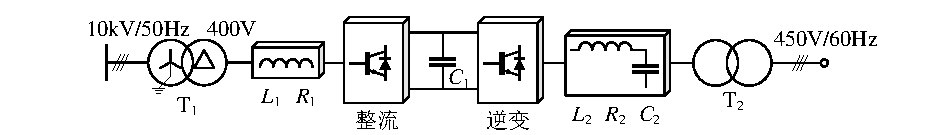
\includegraphics[width=\textwidth]{chapter3/低压岸电换流系统仿真结构示意图.pdf}
	\caption{仿真结构示意图}
	\label{fig:仿真结构示意图}
\end{figure}

\begin{figure}[!htp]
	\centering
	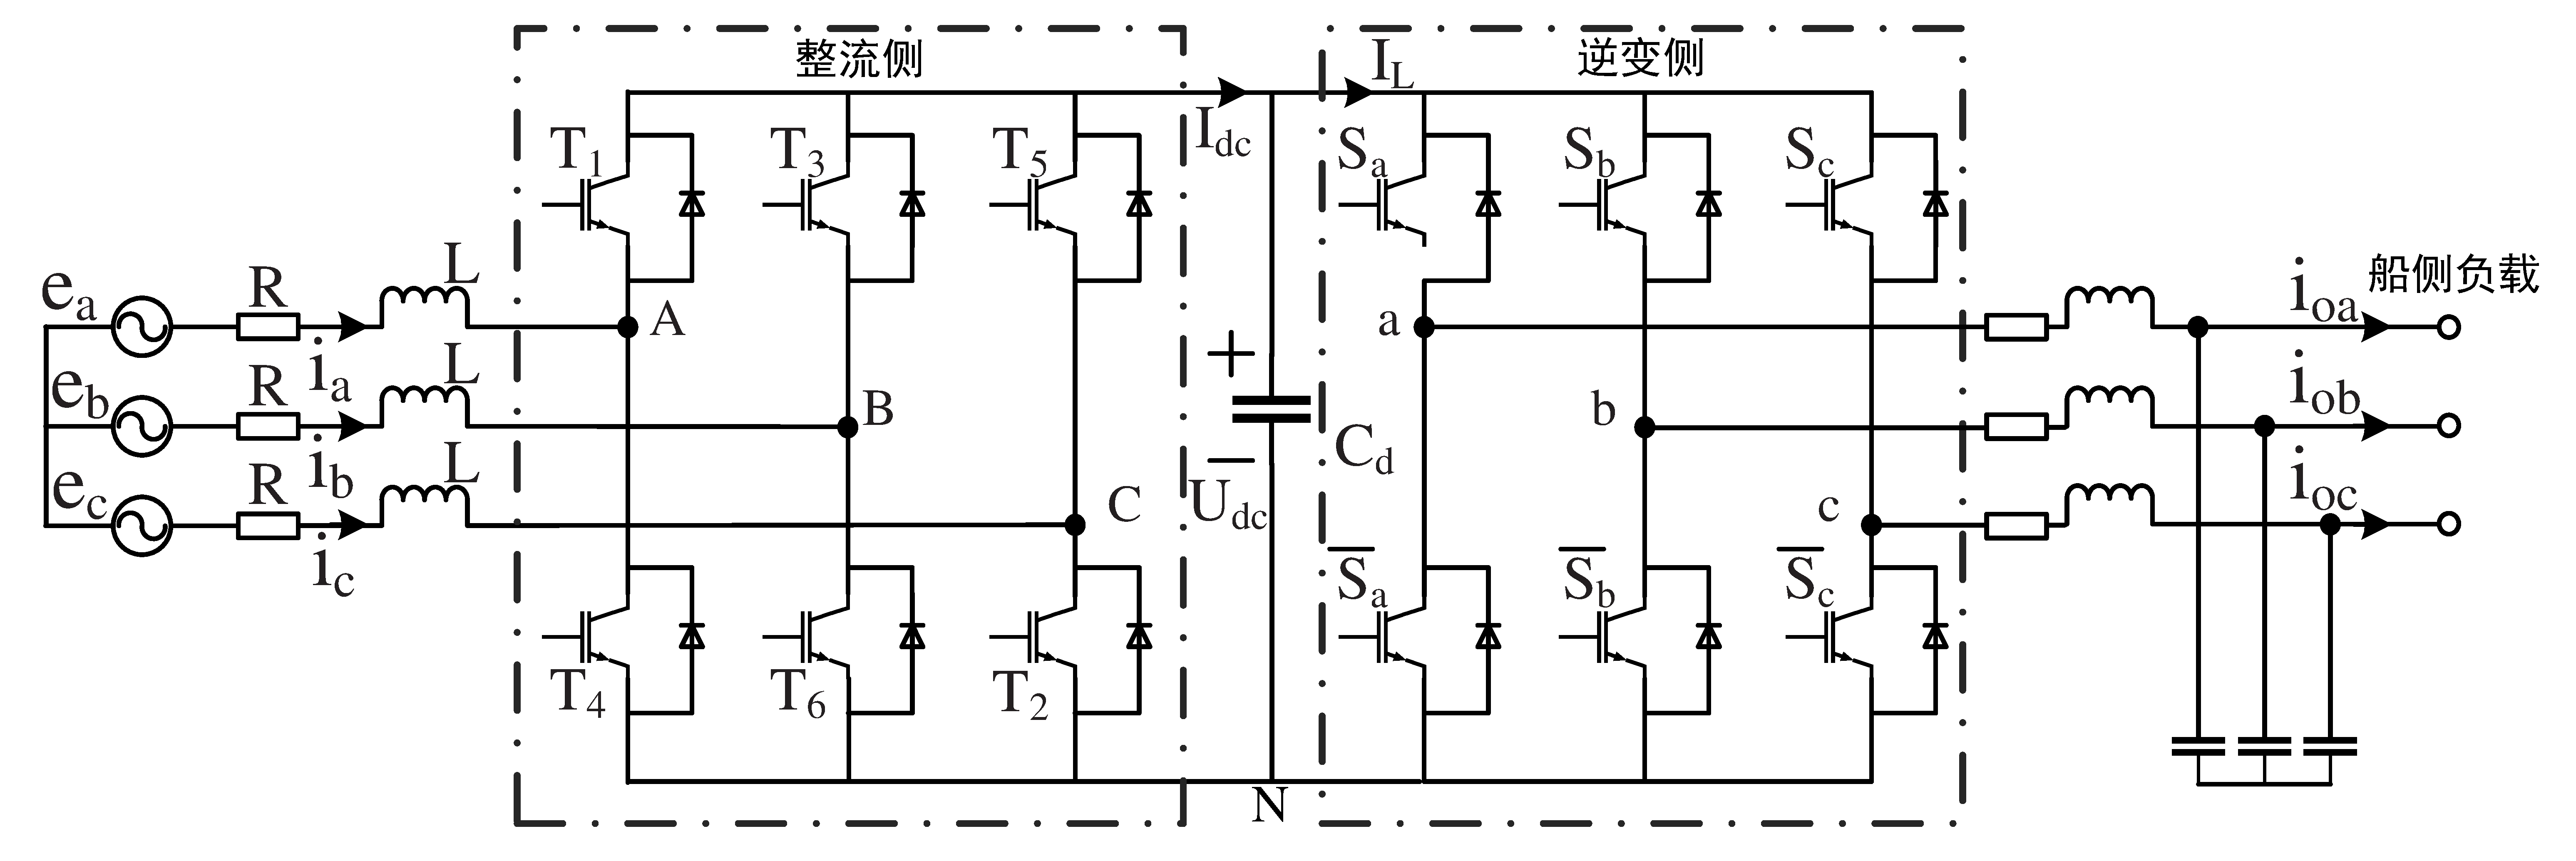
\includegraphics[width=\textwidth]{chapter3/变流器拓扑.pdf}
	\caption{岸电电源变流系统}
	\label{fig:岸电电源变流系统}
\end{figure}



\section{岸侧变流器系统模型与分析}


\subsection{变流器整流侧模型}

\zhlipsum[1]

\begin{figure}[!htp]
	\centering
	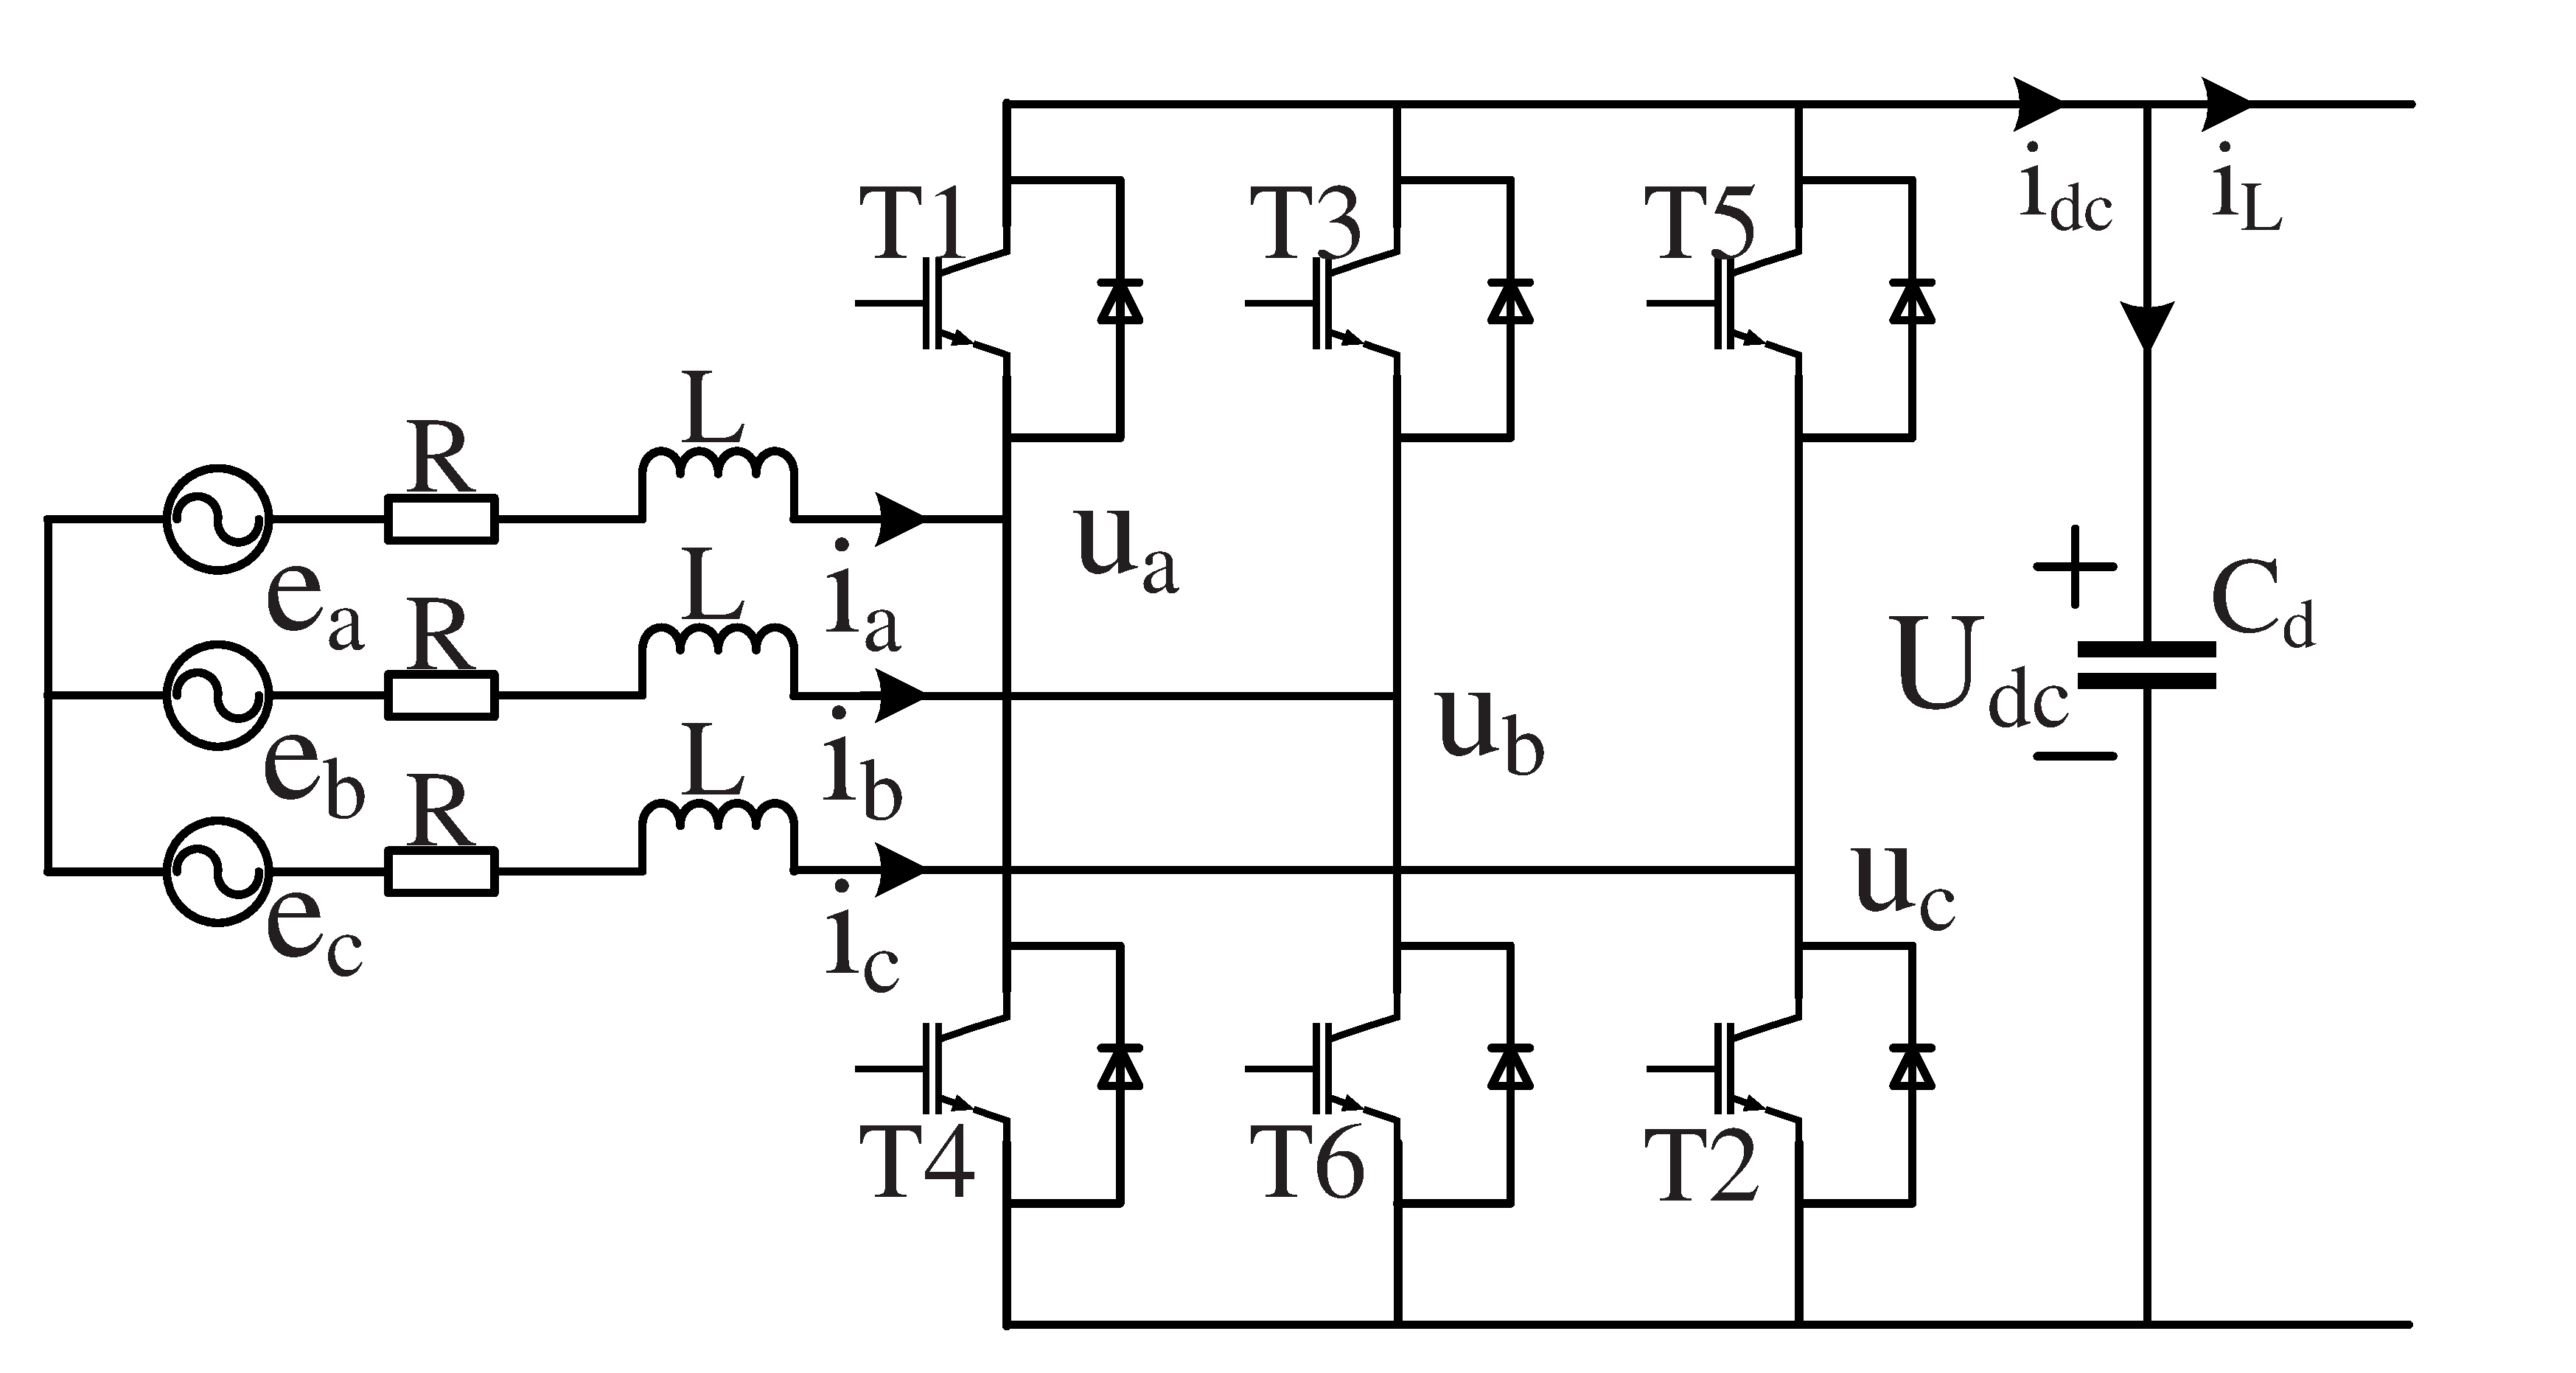
\includegraphics[width=0.65\textwidth]{chapter3/VSR/VSR拓扑.pdf}
	\caption{三相VSR拓扑结构图}
	\label{fig:三相VSR拓扑结构图}
\end{figure}

\begin{equation}
	s_{k} =
	\begin{cases}
		1 \quad \text{上桥臂IGBT导通,下桥臂IGBT关断} \\
		0 \quad \text{上桥臂IGBT关断,下桥臂IGBT导通} \\
	\end{cases}
	(k=a,b,c)
	\label{equ:Sk}
\end{equation}

\begin{equation}
	L\frac{di_{u}}{dt}+Ri_{u}=e_{u}-(u_{uN}+u_{NO})
	\label{equ:3-3}
\end{equation}

\begin{equation}
	L\frac{di_{u}}{dt}+Ri_{u}=e_{u}-(u_{dc}s_{u}+u_{NO})
\end{equation}
同样的v,w相
\begin{equation}
	L\frac{di_{v}}{dt}+Ri_{v}=e_{v}-(u_{dc}s_{v}+u_{NO})
	\label{equ:3-4}
\end{equation}

\begin{equation}
	L\frac{di_{w}}{dt}+Ri_{w}=e_{w}-(u_{dc}s_{w}+u_{NO})
	\label{equ:3-5}
\end{equation}
三相对称,所以有:
\begin{equation}
	e_{u}+e_{v}+e_{w}=0
	\label{equ:3-6}
\end{equation}

\begin{equation}
	i_{u}+i_{v}+i_{w}=0 
	\label{equ:3-7}
\end{equation}
将式(\ref{equ:3-6})式(\ref{equ:3-7})代入式(\ref{equ:3-3})~\~{}式(\ref{equ:3-5})中得:
\begin{equation}
	u_{NO}=-\frac{u_{dc}}{3} \left ( s_{u}+s_{v}+s_{w}  \right )
\end{equation}
直流侧电流$i_{dc}$可以表示为:
\begin{equation}
	i_{dc}=i_{u}s_{u}+i_{v}s_{w}+i_{w}s_{w}
\end{equation}
直流侧电容电流:
\begin{equation}
	C\frac{du_{dc}}{dt}=i_{u}s_{u}+i_{v}s_{w}+i_{w}s_{w}-i_{L}
\end{equation}

设状态变量$\boldsymbol{X}=[i_{u},i_{v},i_{w},u_{dc}]^{T}$,
输入变量$\boldsymbol{U}=[e_{u},e_{v},e_{w},i_{L}]^{T}$则三项VSR状态空间可以表示为:

\begin{equation}
	\boldsymbol{\dot{X}}=\boldsymbol{AX}+\boldsymbol{BU}
\end{equation}
上式中:
\begin{equation}
	\boldsymbol{A}=
	\begin{pmatrix}
		-\frac{R}{L}    & 0               & 0               & -\frac{1}{L}  ( s_{u}-\frac{1}{3} \sum\limits_{k=u,v,w} s_{k}  ) \\
		0               & -\frac{R}{L}    & 0               & -\frac{1}{L}  ( s_{u}-\frac{1}{3} \sum\limits_{k=u,v,w} s_{k}  ) \\
		0               & 0               & -\frac{R}{L}    & -\frac{1}{L}  ( s_{u}-\frac{1}{3} \sum\limits_{k=u,v,w} s_{k}  ) \\
		\frac{s_{a}}{C} & \frac{s_{b}}{C} & \frac{s_{c}}{C} & 0
	\end{pmatrix}
\end{equation}

\begin{equation}
	\boldsymbol{B}=
	\begin{pmatrix}
		\frac{1}{L} & 0           & 0           & 0            \\
		0           & \frac{1}{L} & 0           & 0            \\
		0           & 0           & \frac{1}{L} & 0            \\
		0           & 0           & 0           & -\frac{1}{C}
	\end{pmatrix}
\end{equation}
三相VSR的数学模型结构如图\ref{fig:三相VSR一般数学模型结构}所示:

\begin{figure}[!htp]
	\centering
	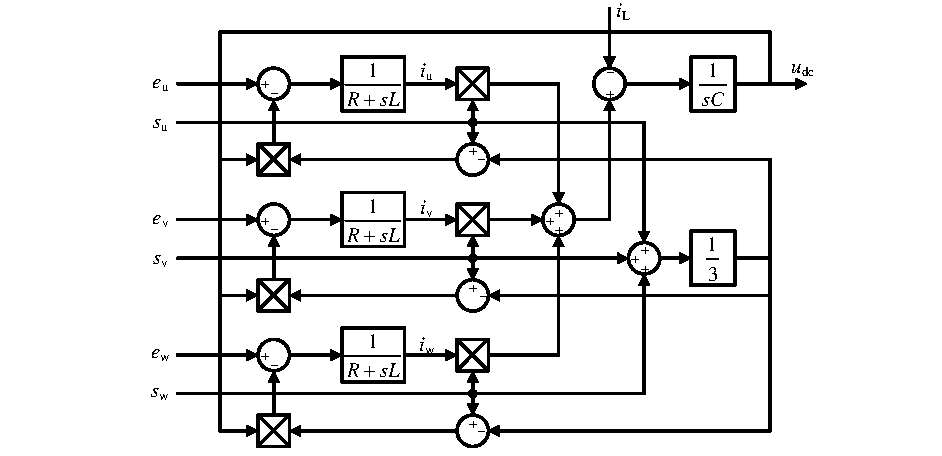
\includegraphics[width=\textwidth]{chapter3/VSR/三相VSR一般数学模型结构.pdf}
	\caption{三相VSR一般数学模型结构}
	\label{fig:三相VSR一般数学模型结构}
\end{figure}

前文对三相静止abc坐标系中的VSR一般数学模型进行了分析,此模型具有物理意义清晰、直观等特点。
但在一般数学模型中,VSR网侧均为时变交流量,不利于控制系统设计。鉴于此,可以通过坐标变换将三相静止abc
坐标系转换成以网侧电动势基波角频率同步旋转的dq坐标系。坐标变换后,三相交变量转化成同步旋转坐标系中的直流量,
从而简化了控制系统的设计。

为将三相静止abc坐标系转换成同步旋转dq坐标系,首先可将三相静止坐标系转换成两相静止$\alpha\beta$坐标系。
设有通用矢量$\boldsymbol{X}$ ,
其在$\alpha$、$\beta$轴上的投影为$x_{\alpha}$、$x_{\beta}$,在a、b、c轴上的投影为$x_{a}$、$x_{b}$、$x_{c}$,
令a轴与α轴重合,则有:

\begin{equation}
	\begin{pmatrix}
		x_{\alpha } \\
		x_{\beta }
	\end{pmatrix}
	=
	\frac{2}{3}
	\begin{pmatrix}
		1 & -\frac{1}{2}         & -\frac{1}{2}        \\
		0 & -\frac{\sqrt{3} }{2} & \frac{\sqrt{3} }{2}
	\end{pmatrix}
	\begin{pmatrix}
		x_{a} \\
		x_{b} \\
		x_{c}
	\end{pmatrix}
	\label{equ:abc2αβ}
\end{equation}
或
\begin{equation}
	\begin{pmatrix}
		x_{a} \\
		x_{b} \\
		x_{c}
	\end{pmatrix}
	=
	\begin{pmatrix}
		1            & 0                    \\
		-\frac{1}{2} & -\frac{\sqrt{3} }{2} \\
		-\frac{1}{2} & \frac{\sqrt{3} }{2}
	\end{pmatrix}
	\begin{pmatrix}
		x_{\alpha } \\
		x_{\beta }
	\end{pmatrix}
\end{equation}
对于三相VSR有:
\begin{equation}
	\begin{cases}
		x_{k}\in  \{ e_{k},e_{k},s_{k} \} \quad(k=a,b,c)          \\
		x_{l}\in  \{ e_{l},e_{l},s_{l} \} \quad(l=\alpha ,\beta ) \\
		x_{j}\in  \{ e_{j},e_{j},s_{j} \} \quad(j=d,q)
	\end{cases}
\end{equation}
化简,可得两相静止坐标系中三相 VSR 开关函数模型为:
\begin{equation}
	\begin{cases}
		C \frac{\mathrm{d} u_{\mathrm{dc}}}{\mathrm{d} t}=\frac{3}{2}\left(i_{\alpha} s_{\alpha}+i_{\beta} s_{\beta}\right)-i_{\mathrm{L}} \\
		L \frac{\mathrm{d} i_{\alpha}}{\mathrm{d} t}+R i_{\alpha}=e_{\alpha}-u_{\mathrm{dc}} s_{\alpha}                                    \\
		L \frac{\mathrm{d} i_{\beta}}{\mathrm{d} t}+R i_{\beta}=e_{\beta}-u_{\mathrm{dc}} s_{\beta}
	\end{cases}
	\label{equ:3-17}
\end{equation}
两相静止坐标系到同步旋转坐标系的转换矩阵为:
\begin{equation}
	\begin{pmatrix}
		x_{\alpha } \\
		x_{\beta }
	\end{pmatrix}=
	\begin{pmatrix}
		cos\varphi & -sin\varphi \\
		sin\varphi & cos\varphi
	\end{pmatrix}
	\begin{pmatrix}
		x_{d } \\
		x_{q}
	\end{pmatrix}
	\label{equ:αβ2dq变换公式}
\end{equation}
式中,$\varphi$为d轴与$\alpha$轴的夹角。将式(\ref{equ:αβ2dq变换公式})代入式(\ref{equ:3-17}),得到
三相VSR在dq坐标系下的数学模型:
\begin{equation}
	\begin{cases}
		C \frac{\mathrm{d} u_{\mathrm{dc}}}{\mathrm{d} t}=\frac{3}{2}\left(i_{\mathrm{d}} s_{\mathrm{d}}+i_{\mathrm{q}} s_{\mathrm{q}}\right)-i_{\mathrm{L}} \\
		L \frac{\mathrm{d} i_{\mathrm{d}}}{\mathrm{d} t}+R i_{\mathrm{d}}-\omega L i_{\mathrm{q}}=e_{\mathrm{d}}-u_{\mathrm{dc}} s_{\mathrm{d}}              \\
		L \frac{\mathrm{d} i_{\mathrm{q}}}{\mathrm{d} t}+R i_{\mathrm{q}}+\omega L i_{\mathrm{d}}=e_{\mathrm{q}}-u_{\mathrm{dc}} s_{\mathrm{q}}
	\end{cases}
	\label{equ:VSR dq数学模型}
\end{equation}

\begin{figure}[!htp]
	\centering
	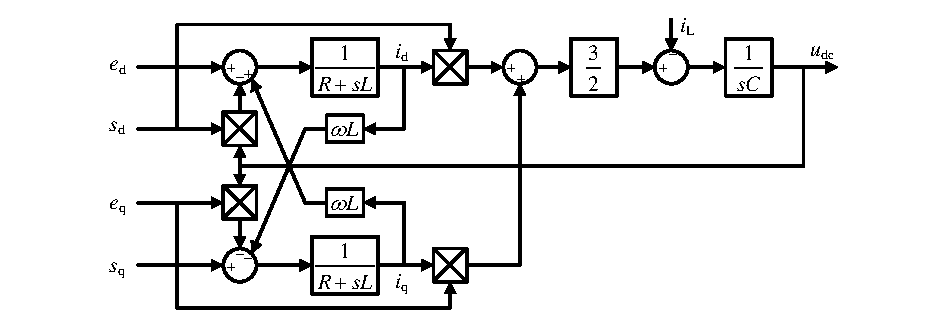
\includegraphics[width=\textwidth]{chapter3/VSR/三相VSR dq数学模型结构.pdf}
	\caption{三相VSR dq数学模型结构.pdf}
	\label{fig:三相VSR dq数学模型结构.pdf}
\end{figure}

\subsection{变流器逆变侧模型}

\begin{figure}[!htp]
	\centering
	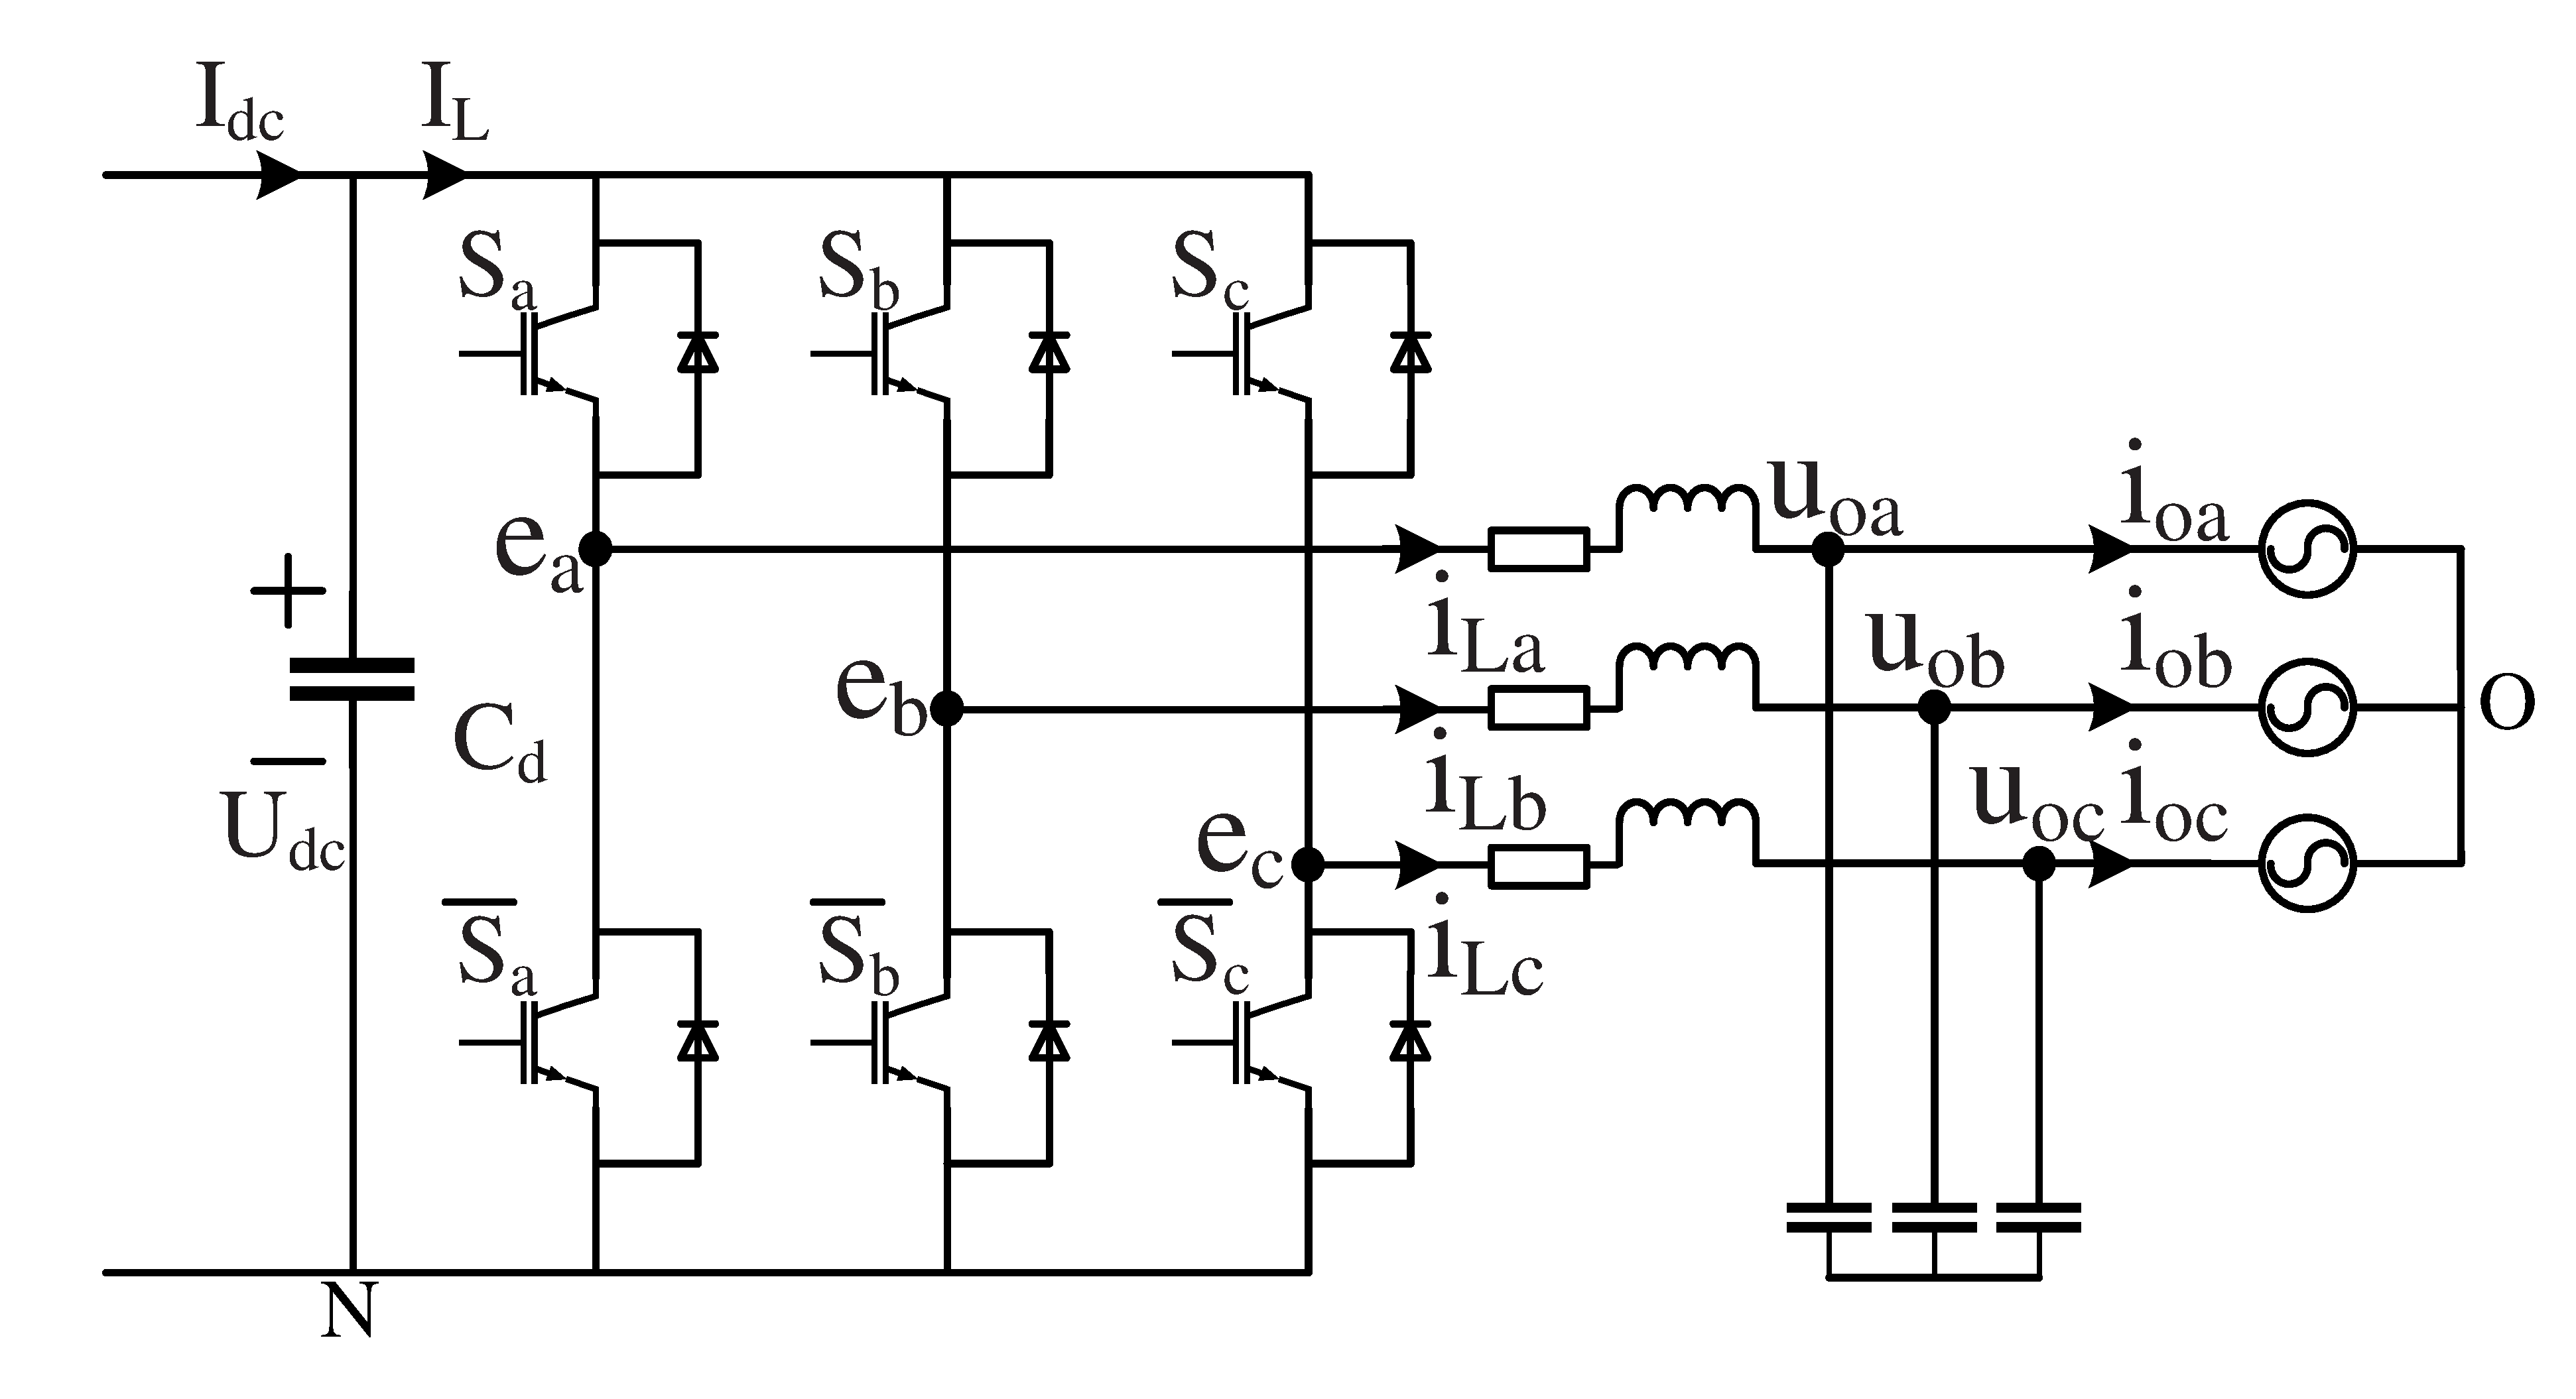
\includegraphics[width=0.65\textwidth]{chapter3/VSI/VSI拓扑.pdf}
	\caption{三相VSI拓扑结构图}
	\label{fig:三相VSI拓扑结构图}
\end{figure}
同三相 VSR 一样,首先定义单极性二值逻辑开关函数$s_{k}$为:
\begin{equation}
	s_{j} =
	\begin{cases}
		1 \quad \text{上桥臂IGBT导通,下桥臂IGBT关断} \\
		0 \quad \text{上桥臂IGBT关断,下桥臂IGBT导通} \\
	\end{cases}
	(j=a,b,c)
	\label{equ:Sk}
\end{equation}
根据基尔霍夫电压定律建立三相VSI回路方程:
\begin{equation}
	\begin{cases}
		L \frac{d i_{La}}{dt}+R i_{La}=e_{a}-u_{oa}-u_{ON} \\
		L \frac{d i_{Lb}}{dt}+R i_{Lb}=e_{b}-u_{ob}-u_{ON} \\
		L \frac{d i_{Lc}}{dt}+R i_{Lc}=e_{c}-u_{oc}-u_{ON}
	\end{cases}
	\label{equ:3-21}
\end{equation}
将$e_{k}=u_{dc}s_{k}\quad(k=a,b,c)$代入式(\ref{equ:3-21})得:
\begin{equation}
	\begin{cases}
		L\frac{di_{La}}{dt}+Ri_{La}=u_{dc}s_{a}-u_{oa}-u_{ON} \\
		L\frac{di_{Lb}}{dt}+Ri_{Lb}=u_{dc}s_{b}-u_{ob}-u_{ON} \\
		L\frac{di_{Lc}}{dt}+Ri_{Lc}=u_{dc}s_{c}-u_{oc}-u_{ON}
		\label{equ:VSI model1}
	\end{cases}
\end{equation}
考虑到三相对称性,则有:
\begin{equation}
	i_{La}+i_{Lb}+i_{Lc}=0 \quad u_{oa}+u_{ob}+u_{oc}=0 \label{equ:3-23}
\end{equation}
联立式(\ref{equ:VSI model1})和式(\ref{equ:3-23})得:
\begin{equation}
	u_{ON}=\frac{u_{dc}}{3}\sum_{k=a,b,c}s_{k}
\end{equation}
根据基尔霍夫电流定律建立整流侧电容电流方程和滤波电容节点处电流方程:
\begin{equation}
	\begin{cases}
		C\frac{du_{oa}}{dt}=i_{La}-i_{oa} \\
		C\frac{du_{ob}}{dt}=i_{Lb}-i_{ob} \\
		C\frac{du_{oc}}{dt}=i_{Lc}-i_{oc} \\
		C\frac{du_{dc}}{dt}=i_{dc}-i_{L}
	\end{cases}
\end{equation}

设状态变量$\boldsymbol{X}=[i_{La},i_{Lb},i_{Lc},u_{dc}]^{T}$,
输入变量$\boldsymbol{U}=[e_{oa},e_{ob},e_{oc},i_{L}]^{T}$则三项VSR状态方程可以表示为:
\begin{equation}
	\boldsymbol{\dot{X}}=\boldsymbol{A}\boldsymbol{X}+\boldsymbol{B}\boldsymbol{E}+\boldsymbol{Z}
\end{equation}
上式中:
\begin{equation}
	\boldsymbol{A}=
	\begin{pmatrix}
		-\frac{R}{L}    & 0               & 0               & - \frac{1}{3L} \sum\limits_{k=u,v,w} s_{k} \\
		0               & -\frac{R}{L}    & 0               & - \frac{1}{3L} \sum\limits_{k=u,v,w} s_{k} \\
		0               & 0               & -\frac{R}{L}    & - \frac{1}{3L} \sum\limits_{k=u,v,w} s_{k} \\
		\frac{s_{a}}{C} & \frac{s_{b}}{C} & \frac{s_{c}}{C} & 0
	\end{pmatrix}
\end{equation}

\begin{equation}
	\boldsymbol{B}=
	\begin{pmatrix}
		-\frac{1}{L} & 0            & 0            & 0            \\
		0            & -\frac{1}{L} & 0            & 0            \\
		0            & 0            & -\frac{1}{L} & 0            \\
		0            & 0            & 0            & -\frac{1}{C}
	\end{pmatrix}
\end{equation}

\begin{equation}
	\boldsymbol{Z}=
	\begin{pmatrix}
		0 & 0 & 0 & \frac{i_{dc}}{C}
	\end{pmatrix}^{T}
\end{equation}

与整流侧类似,为了得到三相VSI dq数学模型,新疆abc静止坐标系转换为两相静止$\alpha\beta$坐标系。
结合式(\ref{equ:abc2αβ})与式(\ref{equ:VSI model1})得到三相VSI$\alpha\beta$模型:
\begin{equation}
	\begin{cases}
		L\frac{di_{L\alpha}}{dt}=-Ri_{L\alpha}+e_{\alpha}-u_{o\alpha} \\
		L\frac{di_{L\beta}}{dt}=-Ri_{L\beta}+e_{\beta}-u_{o\beta}
	\end{cases}
	\label{equ:VSI αβ model1}
\end{equation}

\begin{equation}
	\begin{cases}
		C\frac{du_{o\alpha}}{dt}=i_{L\alpha}-i_{o\alpha} \\
		C\frac{du_{o\beta}}{dt}=i_{L\beta}-i_{o\beta}
	\end{cases}
	\label{equ:VSI αβ model2}
\end{equation}

为使两相静止$\alpha\beta$坐标系转化为同步旋转dq坐标系,将式(\ref{equ:αβ2dq变换公式})代入
式(\ref{equ:VSI αβ model1})和式(\ref{equ:VSI αβ model2})中,整理得到VSI dq模型:
\begin{equation}
	\begin{cases}
		L\frac{di_{Ld}}{dt}=-Ri_{Ld}+e_{d}+\omega Li_{Lq}-u_{od} \\
		L\frac{di_{Lq}}{dt}=-Ri_{Lq}+e_{q}-\omega Li_{Ld}-u_{oq}
	\end{cases}
	\label{equ:VSI dq model1}
\end{equation}

\begin{equation}
	\begin{cases}
		C\frac{du_{od}}{dt}=i_{Ld}+\omega Cu_{oq}-i_{od} \\
		C\frac{du_{oq}}{dt}=i_{Ld}-\omega Cu_{oa}-i_{oq}
	\end{cases}
	\label{equ:VSI dq model2}
\end{equation}

三相VSI dq模型结构,如图\ref{fig:两相同步旋转dq坐标系中三相VSI模型结构图}所示。

\begin{figure}[!htp]
	\centering
	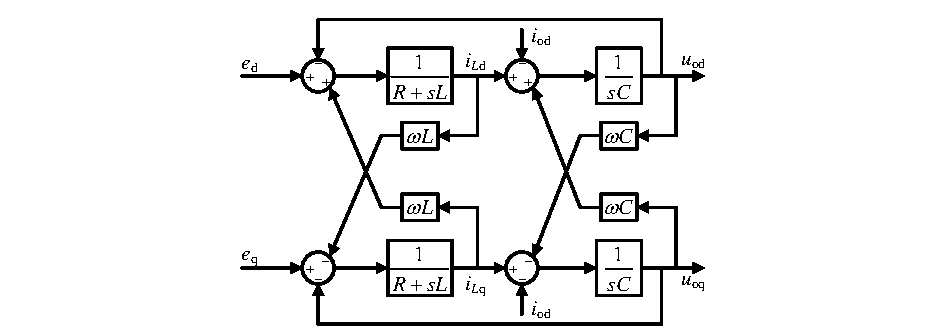
\includegraphics[width=\textwidth]{chapter3/VSI/两相同步旋转坐标系中三相VSI模型结构图.pdf}
	\caption{两相同步旋转dq坐标系中三相VSI模型结构图}
	\label{fig:两相同步旋转dq坐标系中三相VSI模型结构图}
\end{figure}

\section{岸侧变流器系统控制策略}

\subsection{变流器整流侧控制方法}

\zhlipsum[3]

\begin{figure}[!htp]
	\centering
	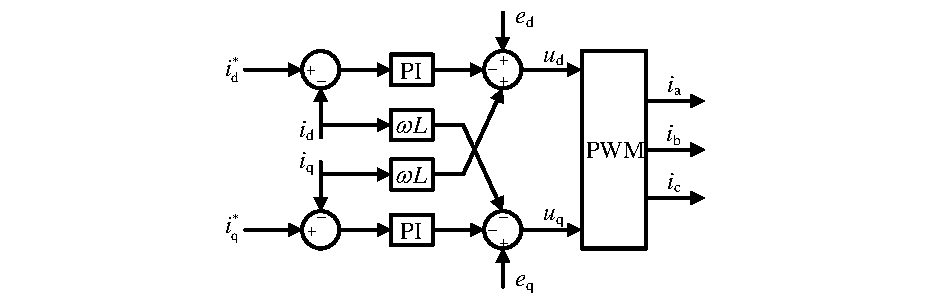
\includegraphics[width=\textwidth]{chapter3/VSR/三相VSR电流内环解耦控制结构.pdf}
	\caption{三相VSR电流内环解耦控制结构}
	\label{fig:三相VSR电流内环解耦控制结构}
\end{figure}

\begin{figure}[!htp]
	\centering
	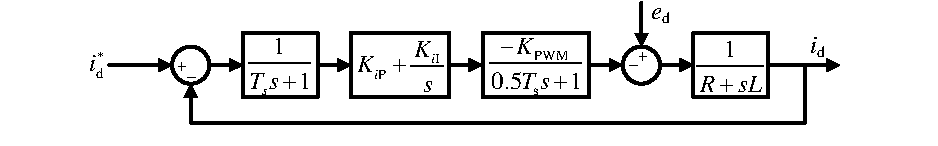
\includegraphics[width=\textwidth]{chapter3/VSR/id电流内环结构.pdf}
	\caption{id电流内环结构}
	\label{fig:id电流内环结构}
\end{figure}

\begin{figure}[!htp]
	\centering
	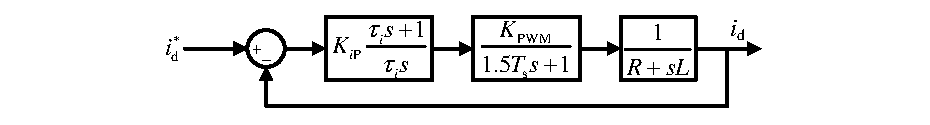
\includegraphics[width=\textwidth]{chapter3/VSR/无ed扰动时的id电流内环结构.pdf}
	\caption{无ed扰动时的id电流内环结构.pdf}
	\label{fig:无ed扰动时的id电流内环结构.pdf}
\end{figure}

\begin{figure}[!htp]
	\centering
	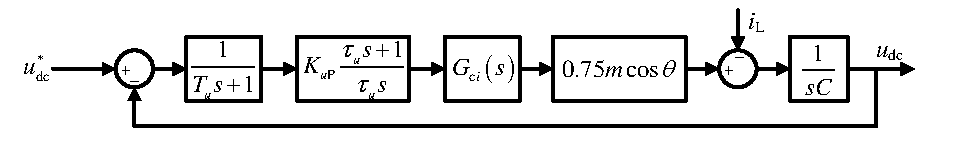
\includegraphics[width=\textwidth]{chapter3/VSR/三相VSR电压外环控制结构.pdf}
	\caption{三相VSR电压外环控制结构}
	\label{fig:三相VSR电压外环控制结构}
\end{figure}

\begin{figure}[!htp]
	\centering
	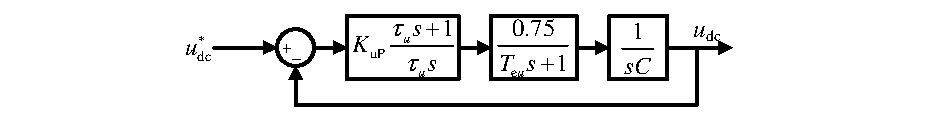
\includegraphics[width=\textwidth]{chapter3/VSR/三相VSR电压外环简化结构.pdf}
	\caption{三相VSR电压外环简化结构}
	\label{fig:三相VSR电压外环简化结构}
\end{figure}

\subsection{变流器逆变侧控制方法}

\zhlipsum[3]

\begin{figure}[!htp]
	\centering
	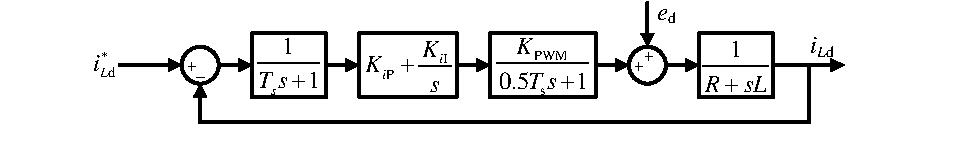
\includegraphics[width=\textwidth]{chapter3/VSI/iLd电流内环结构.pdf}
	\caption{iLd电流内环结构}
	\label{fig:iLd电流内环结构}
\end{figure}

\begin{figure}[!htp]
	\centering
	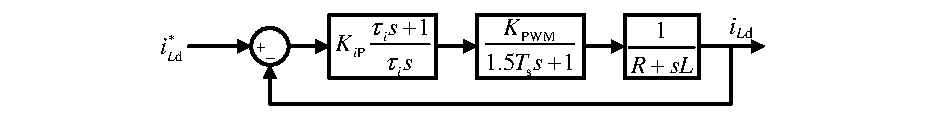
\includegraphics[width=\textwidth]{chapter3/VSI/无ed扰动时的iLd电流内环结构.pdf}
	\caption{无ed扰动时的iLd电流内环结构}
	\label{fig:无ed扰动时的iLd电流内环结构}
\end{figure}

\begin{figure}[!htp]
	\centering
	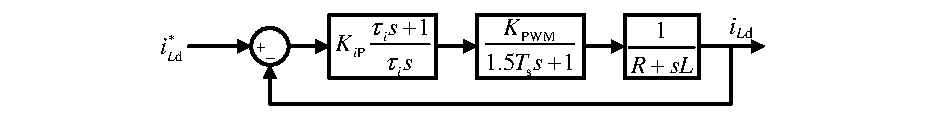
\includegraphics[width=\textwidth]{chapter3/VSI/Uod电压外环结构.pdf}
	\caption{Uod电压外环结构}
	\label{fig:Uod电压外环结构}
\end{figure}

\begin{figure}[!htp]
	\centering
	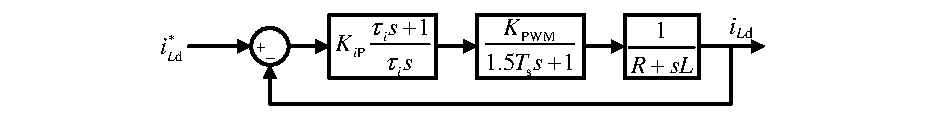
\includegraphics[width=\textwidth]{chapter3/VSI/Uod电压外环简化结构.pdf}
	\caption{Uod电压外环简化结构}
	\label{fig:Uod电压外环简化结构}
\end{figure}


\section{岸侧变压器数学模型}


\section{岸侧滤波器数学模型}


\section{船岸连接系统仿真模型}


\section{本章小结}